\chapter{A short word on random numbers}
\label{chap:Random numbers}
\begin{figure}[h!]
  \centering
  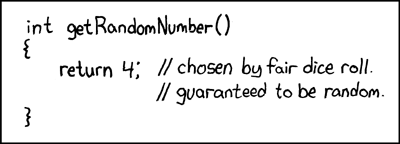
\includegraphics[width=0.4\textwidth]{figures/random_number.png}

  \hspace*{\fill}---Randall Munroe (\href{http://xkcd.com/221/}{XKCD})
\end{figure}
When generating random numbers, you'll want to take care in the methods you use; some RNGs are most definitely better than others.
You can always code your own, but Fortran has a few reasonably good subroutines to do it for you.
The default \texttt{gfortran} installation provides access to a low-level \texttt{\keyword{rand}()} function, but you'll almost certainly want to use the more sophisticated \keyword{random\_number} subroutine instead; it generates much higher quality random numbers and automatically threads over (fills) arrays.
When you've ironed out your algorithm and want to start collecting data, you should also remember to seed the RNG.
Computers generate random numbers by way of a proceedural mathematical formula, so using the same seed produces the same series of random values.
The subroutine in \autoref{lst:init_random_seed} will seed the RNG with entropy collected by the system if it's available, otherwise it will use the current time \& process ID.
\lstinputlisting[float=htbp,label=lst:init_random_seed]{examples/init_random_seed.f90}

The Fortran random number generator produces uniformly distributed reals on the interval\footnote{Be careful with operations that might fail with \texttt{0.0d0}.} $\left[0, 1\right)$, but simulations often require numbers drawn from a different distribution. 
For this, we again turn you to \emph{Numerical Recipes}; it has several means of generating nonuniform random deviates including rejection sampling for Gamma, Poisson, and Binomial distributions and the Box-Muller transform for normal distributions. 
